% !TEX root = thesis.tex
\chapter{深層学習の実装例とその検証}
4章では、NVIDIAのGeForceシリーズの一定性能以上のGPUを搭載したマシンにて、深層学習ライブラリPylearn2やDeep Learning Tutorialを用いた実装を用いることで、深層学習の問題点3つのうち、2つを解決できることを示した。しかし、「分類精度の再現性」の問題については、 実際に実験を行わないとわからないため、保留していた。\par
この章では、実際にPylearn2とDeep Learning Tutorialに実装されている深層学習モデルを用いて、機械学習のタスクを実行する。ここで実際の分類精度を測定することにより、「分類精度の再現の問題」の検証を行う。また、GPUの利用により、どこまで「学習時間の問題」が解消されたのかもチェックする。

\section{実験に利用したデータセット}
実験の前提知識として、この節では、実験に使用したデータセットについて記す。機械学習の分野では、分類精度のベンチマークを取るために、様々なデータセットが提供/提案されてきている。同じデータセットに対して、様々な分類モデルやアルゴリズムを用いて分類実験を行うことにより、どの手法が優れているのか比較することが出来る。\par
ここでは、画像認識のデータセットを用いて、深層学習プログラムのベンチマークを行う。画像データを用いる理由は、1つには、画像認識が深層学習が最も高い分類性能を実現している分野だからである。加えて、画像データや画像から抽出された素性は、可視化が比較的容易なことが多い。可視化することで、学習過程を目で見て確かめることが出来るため、アルゴリズムの分析を行いやすい、という利点がある。
\subsection{MNIST}
MNIST database\footnote{http://yann.lecun.com/exdb/mnist/}とは、手書き数字を画像分析によって認識するベンチマークタスクである。このデータセットは、National Institute of Standards and Technology(NIST)が提供する手書き数字のデータにサイズの規格化処理を加え、数字の書き手毎に整理したものである。データはサイズ28x28ピクセルの白黒画像70000件より構成される\cite{lecun1998gradient-based}。それぞれの画像は、0〜9のいずれかの数字1文字に該当している。画像データを認識プログラムに入力して、どの数字に該当するか判別させることで、画像識別の精度を競うことになる。図\ref{c5_mnist_ex}に、MNISTの画像データの一部を示す。\par
MNISTの70000件のデータは、60000件のモデル訓練用データと、10000件の精度測定用データに分かれている。まず60000件のデータを使って識別モデルに学習を行わせた後、未知の10000件のテストデータを実際に識別してみることで、精度を測定する。テストデータを識別している最中に、更なる学習を行うことは許されない。分類器は、過去に学習に使ったデータだけ良く識別できても意味がなく、むしろ未知のデータこそ精度良く分類出来なければならない。モデルが過去のデータに特化してしまうと、かえって未知のデータに対する識別精度が低下することもある。この低下現象は過学習(over fitting)と呼ばれ、機械学習における落とし穴の一つとなっている。MNISTに限らず、機械学習用のデータセットにて、訓練データとテストデータをあらかじめ分けておくことは一般的であり、学習アルゴリズムが過学習を防げているかどうか、判定するために有効な方法の1つとして知られている。\par
\begin{figure}[tbp]
 \begin{center}
  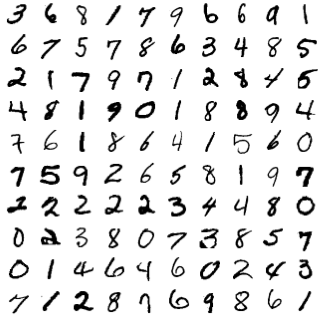
\includegraphics[width=50mm]{img/c5/mnist_ex}
 \end{center}
 \caption{MNISTデータの例(\cite{lecun1998gradient-based}より引用)}
 \label{c5_mnist_ex}
\end{figure}
MNISTは、様々な画像認識アルゴリズムの作者によって使用されている。MNISTの配布ウェブサイトには、MNISTを利用した論文のリストが、分類誤差によるランキング形式で掲載されている。表\ref{c5_mnist_rank}に、MNISTデータセットにおける各アルゴリズムの分類誤差を、ランキング形式のウェブサイト\footnote{\label{c5_rank}\url{http://rodrigob.github.io/are_we_there_yet/build/classification_datasets_results.html}}より再構成して示す。このウェブサイトでは、最新論文に基づく各種データセットの分類誤差ランキングがまとめられている。管理はフェデリコサンタマリア工科大のRodrigo Benenson氏によって行われている\footnote{\url{http://rodrigob.github.io}}。

% Table generated by Excel2LaTeX from sheet 'c5mnist'
\begin{table}[htbp]
\begin{center}
  %\centering
  \caption{MNISTの分類誤差ランキング}
% !TEX root = thesis.tex
    \begin{tabular}{|p{7cm}|p{5cm}|r|}\hline
%    \toprule
    手法 & 発表学会/雑誌/年 & 分類誤差 \\ \hline
%    \midrule
    DropConnect \cite{wan2013regularization}& ICML 2013 & 0.21\% \\ \hline
    Multi-column Deep NN \cite{ciresan2012multi-column}& CVPR 2012 & 0.23\% \\ \hline
    Deep Big Simple Neural Nets \cite{ciresan2010deep}& Neural Computation 2010 & 0.35\% \\ \hline
    Energy-based Model\cite{ranzato2006efficient}& NIPS 2006 & 0.39\% \\ \hline
    CNN \cite{simard2003best}& Document Analysis and Recognition 2003 & 0.40\% \\ \hline
    \textbf{Maxout Networks} \cite{goodfellow2013maxout}& ICML 2013 & 0.45\% \\ \hline
    COSFIREフィルタ \cite{azzopardi2013trainable}& PAMI 2013 & 0.52\% \\ \hline
    Multi-Stage Architecture \cite{jarrett2009what}& ICCV 2009 & 0.53\% \\ \hline
    Deformation Models \cite{keysers2007deformation}& PAMI 2007 & 0.54\% \\ \hline
    A trainable feature extractor \cite{lauer2007a-trainable}& Journal Pattern Recognition 2007   & 0.54\% \\ \hline
    不変SVM \cite{decoste2002training}& Machine Learning 2002 & 0.56\% \\ \hline
    Sparse Coding \cite{labusch2008simple}& TNN 2008 & 0.59\% \\ \hline
    unsupervised learning of invariant feature hierarchies \cite{ranzato2007unsupervised}& CVPR 2007 & 0.62\% \\ \hline
    shape contexts \cite{belongie2002shape}& PAMI 2002 & 0.63\% \\ \hline
    Receptive Field Learning \cite{jia2012beyond}& CVPR 2012 & 0.64\% \\ \hline
    Sparse Activity, Sparse Connectivity \cite{thom2013sparse}& JMLR 2013 & 0.75\% \\ \hline
    Convolutional DBN \cite{lee2009convolutional}& ICML 2009 & 0.82\% \\ \hline
    深層符号器ネットワーク \cite{min2009large-margin}& 2009 & 0.94\% \\ \hline
    深層ボルツマンマシン \cite{salakhutdinov2009deep}& AISTATS 2009 & 0.95\% \\ \hline
    DBN \cite{dahl2008cs81:}& 2008 & 1.12\% \\ \hline
    CNN  \cite{simard2003best}& 2003 & 1.19\% \\ \hline
    ニューラルネットワーク \cite{hinton2006reducing}& 2006 & 1.20\% \\ \hline
    Deep learning via semi-supervised embedding \cite{weston2012deep}& 2008 & 1.50\% \\ \hline
%    \bottomrule
    \end{tabular}%

  \label{c5_mnist_rank}%
  \end{center}
\end{table}%
なお、MNISTのデータによって分類実験をする際、元データを少し歪ませたり、解像度を変更することで入力データの種類を増やすと、良い結果が得られることがわかっている\cite{simard2003best}\cite{lauer2007a-trainable}。一方で、このような元データの変更を禁止した状態で、良い精度を出す試みもある。さらに条件を厳しくして、変形を行わないだけでなく、「2次元の画像データではなく、1次元のベクトルデータである」と考える順序不変(Permutation Invariant, PI)と呼ばれる条件も行われている。このPI条件の場合、2次元的畳み込みネットワークの利用を使うことが出来なくなり、分類精度は大きく落ちることになる。ただ、この条件下でも良い精度を出すことのできるアルゴリズムは、他の1次元のデータ、例えば言語データや音声データにおいても、良い性能を出しやすいと考えられる。今回の実験では、ウェブ工学などへの応用可能性を考えるため、分類モデルが畳み込みレイヤーを含まない場合は、全て順序不変で行っている。畳み込みレイヤーを含むものについては、順序不変にはなっていいが、この場合も元データの変形によるデータ増加は行っていない。

\subsection{CIFAR10}
CIFAR10\footnote{http://www.cs.toronto.edu/~kriz/cifar.html}は、写真を画像分析によって識別するタスクである\cite{krizhevsky2009learning}。入力データは60000件のカラー画像で、どの画像も、飛行機、自動車、鳥、猫、鹿、犬、蛙、馬、船、トラックの10種類のクラスのどれかに属しており、各クラス均等に6000枚ずつの画像が割り振られている。画像データは、GoogleやFlickrなどによるウェブ検索で集められた画像を、人手でラベリングして作られている。また、サイズを32x32ピクセルに縮小されている。\par
MNISTと同じように、60000件のデータは、50000の訓練データと10000件のテストデータに分割されている。まず、分類器にこれらの訓練データを読み取らせて、学習を行わせる。その後、テストデータのうちいくつを正しいクラスに分類することができるのか、分類精度を競うことになる。\par
CIFAR10についても、データの例を図\ref{c5_cifar_ex}に、分類誤差のランキング表を、表\ref{c5_cifar_rank}に示す。このランキングも、MNISTのものと同様に作成されている。
\begin{figure}[tbp]
 \begin{center}
  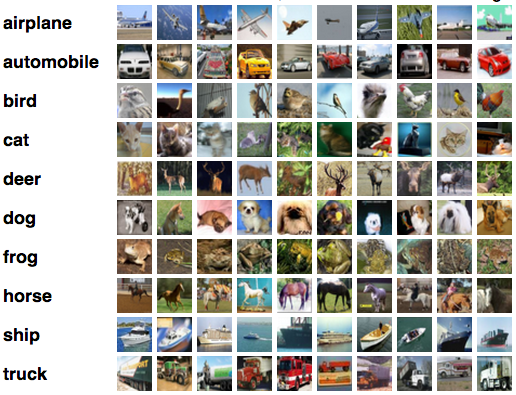
\includegraphics[width=100mm]{img/c5/cifar_ex}
 \end{center}
 \caption{CIFAR10データの例 (http://www.cs.toronto.edu/~kriz/cifar.htmlより引用)}
 \label{c5_cifar_ex}
\end{figure}


\begin{table}[tbp]
 \begin{center}
  \caption{CIFAR10分類誤差のランキング}
   \begin{tabular}{|l|l|r|}\hline
  手法 & 発表学会/雑誌 & 分類誤差 \\ \hline
DropConnect \cite{wan2013regularization}& ICML 2013 & 9.32 \% \\ \hline
Maxout Networks \cite{goodfellow2013maxout}& ICML 2013 & 9.35 \% \\ \hline
Bayesian Optimization \cite{snoek2012practical}& NIPS 2012 & 9.50 \% \\ \hline
深層畳み込みニューラルネットワークworks \cite{krizhevsky2012imagenet}& NIPS 2012 & 11.00 \% \\ \hline
多段深層ニューラルネットワークs \cite{ciresan2012multi-column}& CVPR 2012 & 11.21 \% \\ \hline
深層畳み込みニューラルネットワークworks \cite{zeiler2013stochastic}& arXiv 2013 & 15.13 \% \\ \hline
Dropout \cite{hinton2012improving}& arXiv 2012 & 15.60 \% \\ \hline
Sum-Product Networks \cite{gens2012discriminative}& NIPS 2012 & 16.04 \% \\ \hline
Single-Layer Networks \cite{coates2011an-analysis}& AISTATS 2011 & 20.4 \% \\ \hline
  \end{tabular}

 \end{center}

 \label{c5_cifar_rank}
\end{table}

\section{実験に利用した深層学習のモデル}
ここでは、Pylearn2およびDeep Learning Tutorialに含まれている、深層学習モデルの中で、どのモデルを実験に用いたかを記す。

\subsection{Deep Learning Tutorial内のモデル}
Deep Learning Tutorialからは、CNN\footnote{\url{http://deeplearning.net/tutorial/lenet.html}}、SDA\footnote{\url{http://deeplearning.net/tutorial/SdA.html}}、DBN\footnote{\url{http://deeplearning.net/tutorial/DBN.html}}の3種類の実装を用いた。加えて、CNNの上から2番目のレイヤーを、Dropout + Rectifier Unitに変更したDReDNet\footnote{\url{http://techtalks.tv/talks/drednets/58115/}}と呼ばれるモデルでも実験した。このときユニットの出力を隠す割合を決める破損率(corruption rate)は、0.5に設定した。

\subsection{Pylearn2内のモデル}
Pylearn2からは、CNN\footnote{\url{http://nbviewer.ipython.org/github/lisa-lab/pylearn2/blob/master/pylearn2/scripts/tutorials/convolutional_network.ipynb}}、SDA\footnote{\url{http://nbviewer.ipython.org/github/lisa-lab/pylearn2/blob/master/pylearn2/scripts/tutorials/stacked_autoencoders.ipynb}}、Maxout Network、Maxout+畳み込みレイヤー\footnote{\url{http://deeplearning.net/software/pylearn2/library/models.html\#module-pylearn2.models.maxout}}の4種類のモデルを用いた。DBNについては、構成要素であるRBMの実装は用意されているものの、これを組み立ててDBNにする作業はライブラリの利用者に任されており、完全なソースではないため除外した。

\section{使用したマシンとハードウェア性能}
この章の実験では、2種類のサーバマシンを用いている。一方は、深層学習を目的に構成した自作サーバマシンで、GPUを搭載している(physalisと名付けられている)。もう一方は、Dell社のPowerEdgeT300\footnote{\url{http://www1.jp.dell.com/jp/ja/premier/servers/pedge_t300/pd.aspx?refid=pedge_t300&cs=jppremier1&s=premier}}という機種のもので、こちらにはGPUは搭載されていない(artemisと名付けられている)。表\ref{c5_hardware_spec}に、今回の実験で使用したマシンの主な使用パーツ及び性能を列挙した。また、Pylearn2に実装されているMaxout Networkのソースコードには、実験マシンのパーツ性能を書いたファイルが付属している\footnote{Pylearn2/scripts/papers/maxout/notes}。このファイルの記述内容も、比較のために列挙した。Maxout Networkは、先述したMNISTやCIFAR10のベンチマーク実験において、かなり最先端に高い精度を挙げており、特に順序不変(Permutatin Invariant)のタスクにおいては最も性能が高い。このMaxout Networkの実験に用いられたマシンよりも、ハードウェア面で上回っているならば、ハードウェア面での性能が不足して実験がうまくいかない危険性はかなり低いと言える。今回の実験に使ったマシンで言うと、新しく構成してGPUを搭載したphysalisサーバの方は、論文のマシンよりハードウェア性能的に優れていることがわかる。一方、artemisサーバはGPUを搭載していなかったため、学習速度面にて劣ることが予想される。
\begin{table}[tbp]
 \begin{center}
  \caption{ハードウェア性能の比較}
  \begin{tabular}{|c|c|c|c|c|c|}\hline
  マシン識別名 & GPU & CUDA core & CPU & クロック数 & メモリ容量\\ \hline
physalis & GTX760 & 1152 & Intel CPU Core i7 4770S & 3.1GHz x 8 & 32GB\\ \hline
artemis & (無し) & (無し) & Intel Xeon CPU X3323 & 2.5GHz x 4 & 24GB\\ \hline
(論文) &GTX580 & 512 & Intel Xeon CPU E5620 &  2.4GHz x 4 & (記載無し)\\ \hline
  \end{tabular}
 \end{center}

 \label{c5_hardware_spec}
\end{table}

\section{ベンチマーク実験の詳細}
使用サーバ・ベンチマークセット・ライブラリ・分類モデルの組み合わせについて、分類学習の結果得られる性能を測定した。表\ref{c5_all_result}に結果を示す。ここで、DLTはDeep Learning Tutorial、PL2はPylearn2の略とする。また、PIは、MNISTの実験種類における順序不変タスクのことを指している。この結果に対する考察は、6章にて行う。

% Table generated by Excel2LaTeX from sheet 'summary'
\begin{table}[htbp]
  \centering
  \caption{ベンチマーク実験の結果}
    \begin{tabular}{|c|c|c|c|r|r|r|}\hline
    マシン名 & ライブラリ & データセット & モデル & \shortstack{識別誤差\\(\%)} & \shortstack{実行時間\\(分)} & \shortstack{使用メモリ\\(MB)}\rule[0mm]{0mm}{10mm}\\ \hline
artemis & DLT & CIFAR10 & CNN   & 35.18 & 766   & - \\ \hline
artemis & DLT & CIFAR10 & DBN & 51.01 & 236 &- \\ \hline
artemis & DLT & CIFAR10 & SDA & 56.94 & 1335&- \\ \hline
physalis & DLT & CIFAR10 & CNN & 34.76 & 28&- \\ \hline
physalis & DLT & CIFAR10 & DBN & 50.90& 115 &- \\ \hline
physalis & DLT & CIFAR10 & SDA & 58.64 & 92&- \\ \hline
physalis & DLT & MNIST(PI) & DBN & 1.51& 101 &- \\ \hline
physalis & DLT & MNIST(PI) & SDA & 1.40 & 183 &- \\ \hline
physalis & PL2 & MNIST(PI) & SDA & 1.90 & 128 & 1004 \\ \hline
physalis & PL2 & MNIST(PI) & Maxout & 1.16& 55& 792 \\ \hline
artemis & DLT & MNIST & Drednet & 1.19& 593 &- \\ \hline
physalis & DLT & MNIST & CNN & 0.93& 32&- \\ \hline
physalis & PL2 & MNIST & CNN & 0.68& 30& 796 \\ \hline
physalis & PL2 & MNIST & \shortstack{Maxout\\+畳み込み}\rule[0mm]{0mm}{8mm} & 0.51& 126 & 996 \\ \hline
\end{tabular}%
\label{c5_all_result}%
\end{table}%
\par



\section{その他に行った実験}
ここでは、上記の組み合わせ実験に当てはまらない、独立して行った実験について記す。

\subsection{Maxout Networkによる、MNIST分類の繰り返し実験}
Maxout Networkを利用して、再現精度Pylearn2を利用するにあたり、何らかの原因でランダム性が発生していないか確かめるため、Pylearn2 + Maxout Networkによる、MNISTの順序不変タスク実験を、10回繰り返して行い、分類性能が変化するどうかを見た。乱数のシードは、元論文の実験が行われたときと同じ値で固定した。つまり、乱数以外の原因でランダム性が発生してしまっていないかどうかをチェックした。これは、実験結果の分類誤差が、Maxout Networkの元の論文よりも僅かではあるが悪くなってしまったため、まずアルゴリズムやハードウェアの動作に含まれるランダム性によって、精度が変化してしまっていないことを確かめるためである。\par
実験の結果、誤差は10回とも共通で、1.16\%となった。なお、平均実行時間は約55分、最大メモリ使用量は793MBだった(表\ref{c5_maxout_mnist1_stat})。\par

\begin{table}[tdp]
\caption{Maxout NetworkによるMNIST(1次元)分類タスク繰り返し実験の詳細}
\begin{center}
\begin{tabular}{|c|c|c|}\hline
 & 平均実行時間(秒) & 平均最大使用メモリ(MB) \\ \hline
事前学習 & 2532.8 & 779.3 \\ \hline
微調整 & 756.7 & 792.5 \\ \hline
全体 & 3289.5 & 792.5 \\ \hline
\end{tabular}
\end{center}
\label{c5_maxout_mnist1_stat}
\end{table}%

\section{実験による結論}
この節では、今回の再現実験にて得られた結論について述べる。
\subsection{分類精度の再現性について}
今回の実験で再現出来た分類精度が、データセットの分類精度ランキングの中で、どこに位置づけられるのかを示したのが、表\ref{c5_mnist2_result}及び表\ref{c5_mnist1_result}である。なお、最も性能が高かったMaxout Networkの2つについてのみ示している。特にConvolutional Layerを用いた"2次元、画像変形無し"のタスクで、非常に良い性能を再現できていることがわかる。
\begin{table}[tdp]
\caption{MNIST(2次元、画像変形無し)の分類誤差ランキング(\cite{goodfellow2013maxout}より再構成)}
\begin{center}
    \begin{tabular}{| l | r |}\hline
    手法 & 分類誤差 \\ \hline
    Conv. maxout + dropout & 0.45\% \\ \hline
    Stochastic pooling \cite{zeiler2013stochastic} & 0.47\% \\ \hline
    \textbf{今回の実験} & 0.51\% \\ \hline
2-layer CNN+2-layer NN \cite{jarrett2009what} & 0.53\% \\ \hline
    \end{tabular}%
    \end{center}
\label{c5_mnist2_result}
\end{table}%

\begin{table}[tdp]
\caption{MNIST(1次元、順序不変)の分類誤差ランキング(\cite{goodfellow2013maxout}より再構成)}
\begin{center}
    \begin{tabular}{| l | r |}\hline
    手法 & 分類誤差 \\ \hline
DBM + dropout \cite{hinton2012improving} & 0.79\% \\ \hline
Manifold Tangent Classifier \cite{rifai2011the-manifold} & 0.83\% \\ \hline
Deep Convex Network \cite{yu2011deep} & 0.91\% \\ \hline
Maxout MLP + dropout MP-DBM\cite{goodfellow2012joint} & 0.94\% \\ \hline
DBM \cite{salakhutdinov2009deep} & 0.95\% \\ \hline
Rectifier MLP + dropout \cite{srivastava2013improving} & 1.05\% \\ \hline
\textbf{今回の実験} & 1.16\% \\ \hline
    \end{tabular}%
    \end{center}
\label{c5_mnist1_result}
\end{table}%

\subsection{GPUの利用による学習時間短縮について}
GPUを搭載したphysalisサーバと、搭載していないartemisサーバでDeep Learning Tutorialの3モデルを動かした結果を比較した(表\ref{c5_gpu_result})。2つのマシンはGPUの有無以外にも性能差があるため、一概に比較はできないものの、GPUを搭載しているphysalisマシンの方は、SDAで14.5倍、CNNで27.35倍もの速度上昇を果たしていることがわかる。この2つのモデルについては、GPUを利用することで、4章で挙げた「学習時間の問題」をかなり大きく緩和することが出来ると言える。なお、DBNでは2.05倍の速度上昇に留まっており、深層学習モデルの中でも、GPUの恩恵を受けやすいモデルと、影響が少ないモデルが存在することもわかる。これについては実装による差異も大きいと予想できるので、更なる調査が必要である。\par
なお、DBNとCNNではphysalisマシンの方が誤差が少し小さく、SDAではartemisマシンの方が分類誤差が減少している。これについては、artemisマシンとphysalisマシンでは、実験を行った時期が少しずれているため、numpyなど内部ライブラリのバージョンが異なっている可能性があると考えられる。

\begin{table}[tdp]
\caption{2種類のマシンによるDeep Learning Tutorial+CIFAR10の分類誤差および実行時間}
\centering
\begin{tabular}{|c|c|c|c|c|}\hline
マシン名 & GPU & DBNの結果 & SDAの結果 & CNNの結果\\ \hline
physalis & 有り & 50.90\% ,115分 & 58.64\% ,92分  & 34.76\% ,28分  \\ \hline
artemis & 無し & 51.01\% ,236分 & 56.94\% , 1335分 & 35.18\% ,766分 \\ \hline
\end{tabular}
\label{c5_gpu_result}
\end{table}